\begin{frame}
  \frametitle{Express Parallel Algo independent of processors}
  \begin{figure}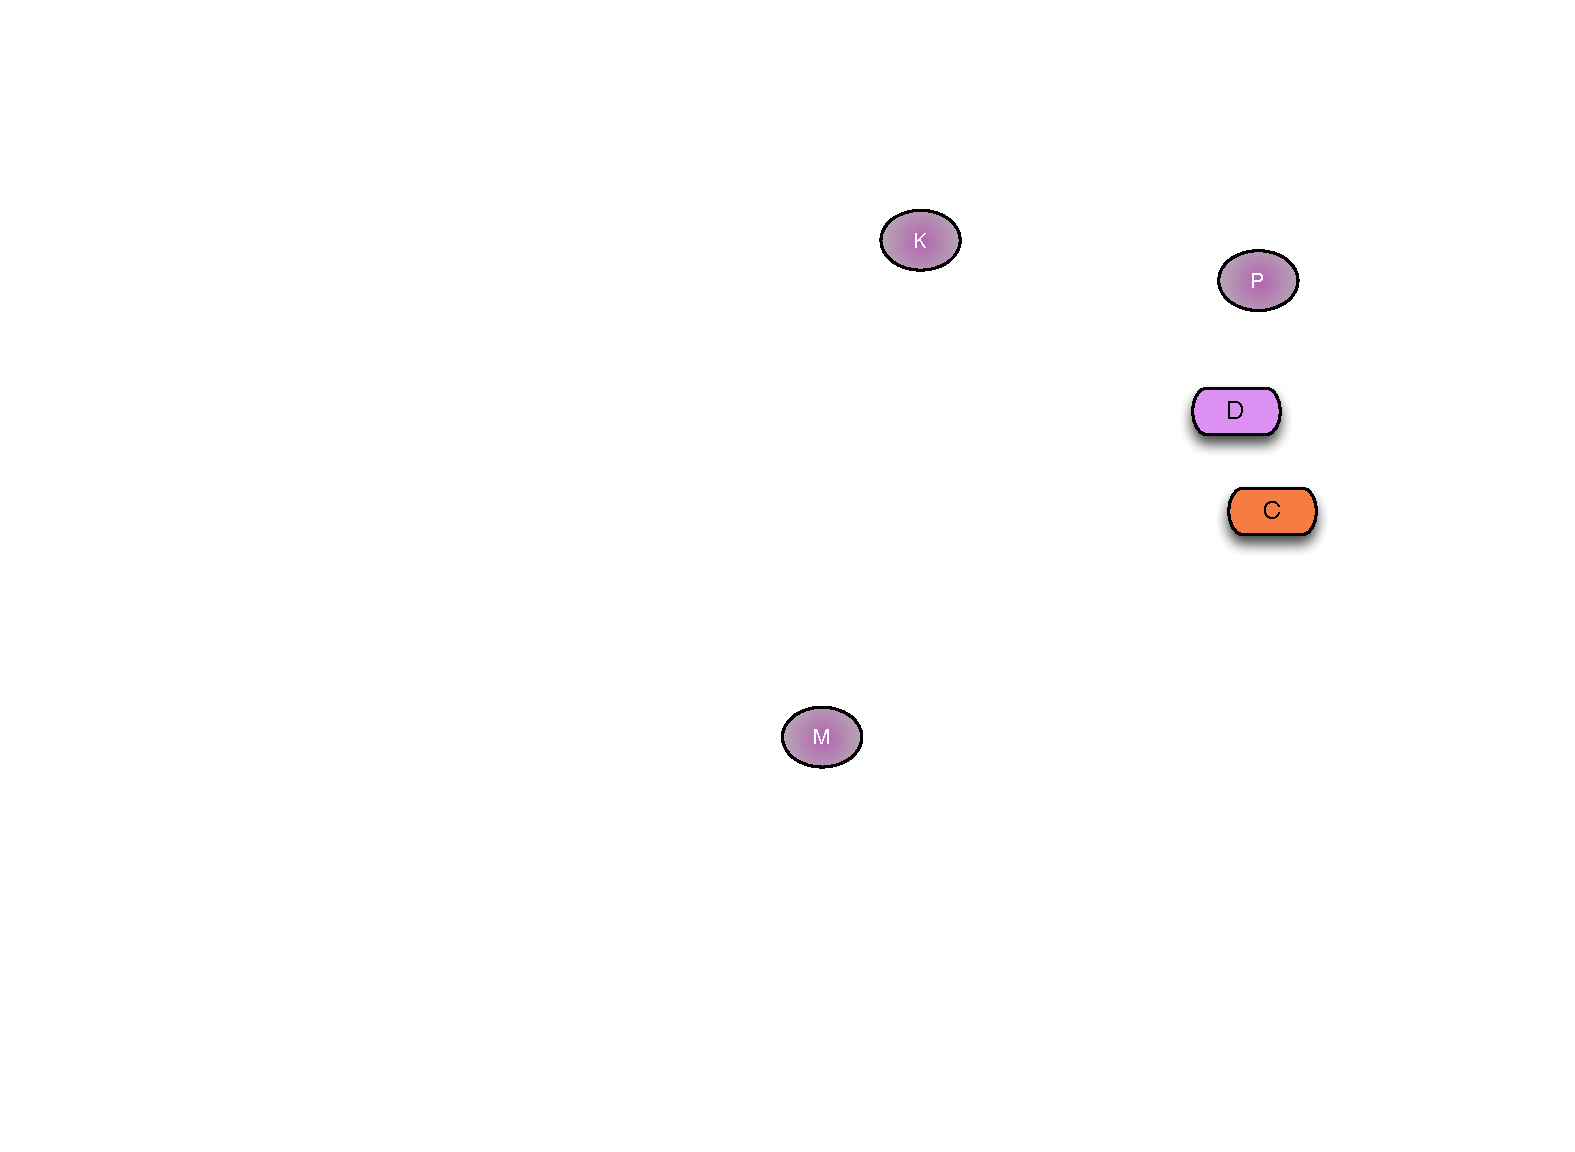
\includegraphics[width=0.9\textwidth]{../figures/progmodel/01-objects-for-algo.pdf}\end{figure}
\end{frame}


\begin{frame}
  \frametitle{Data parallelism: via an Object Collection}
  \begin{figure}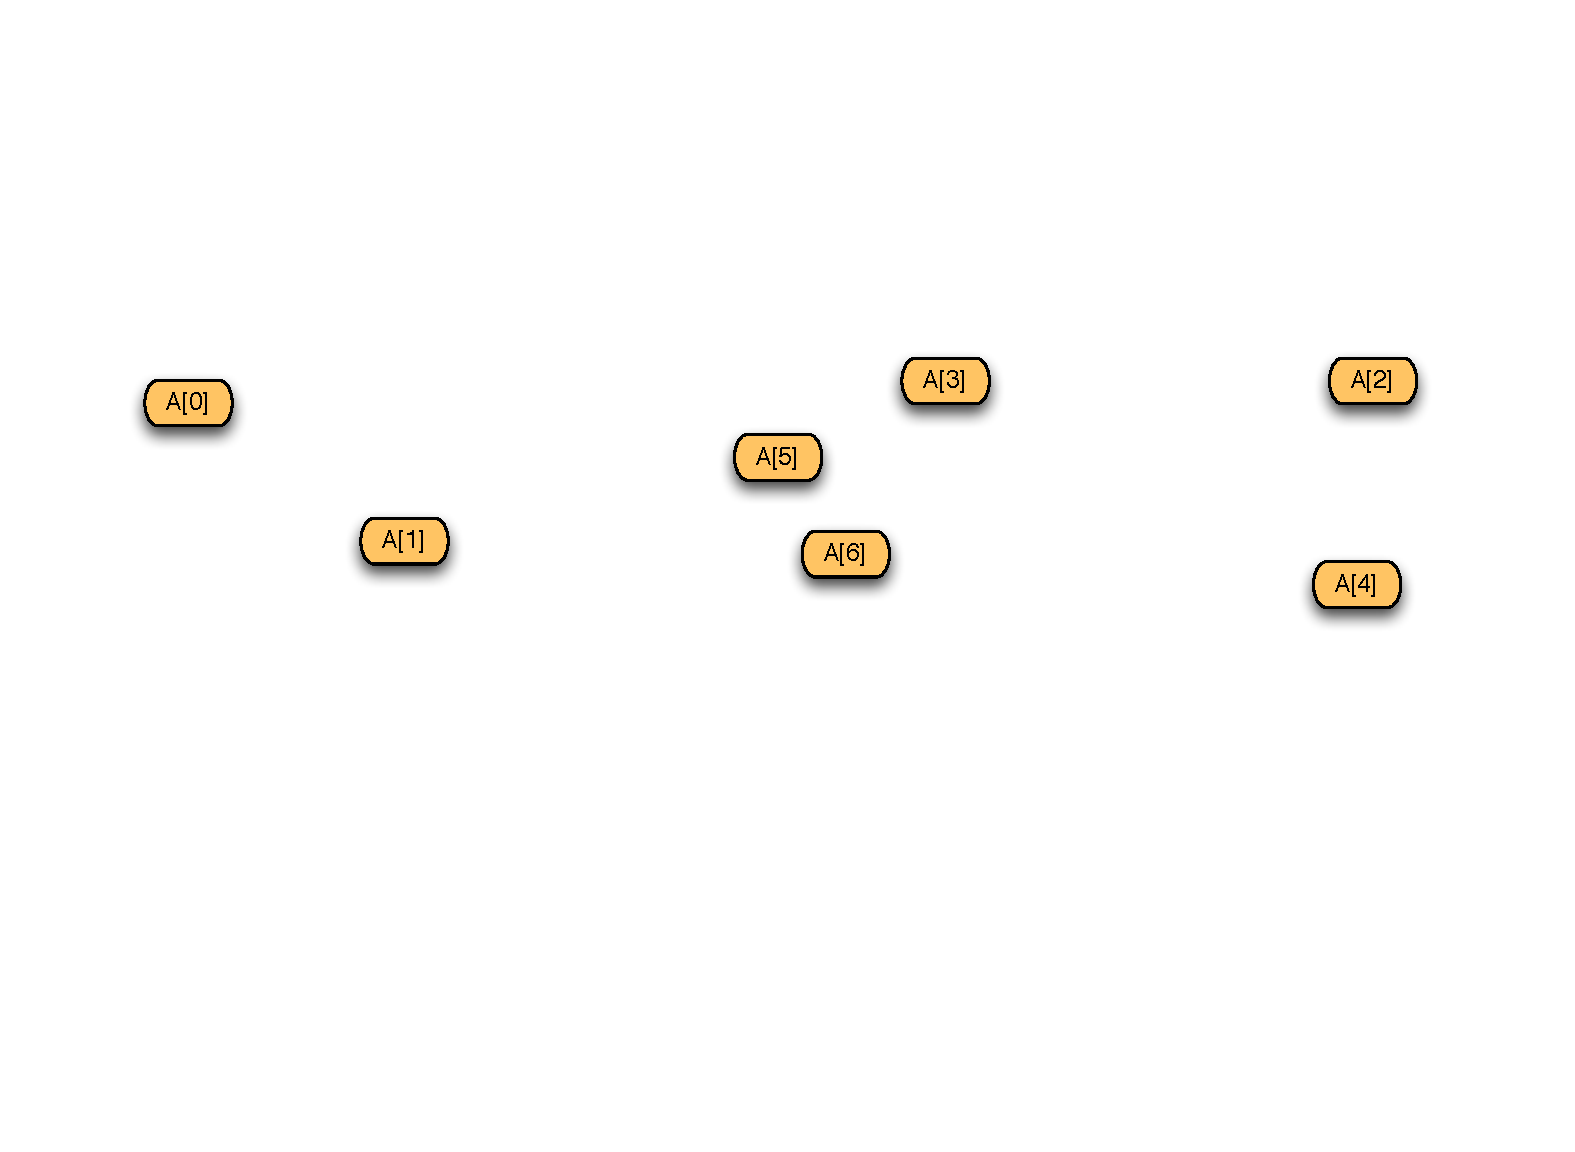
\includegraphics[width=0.9\textwidth]{../figures/progmodel/02-data-decomp-via-arrays.pdf}\end{figure}
\end{frame}


\begin{frame}
  \frametitle{Multiple data parallel collections}
say 2 matrices
  \begin{figure}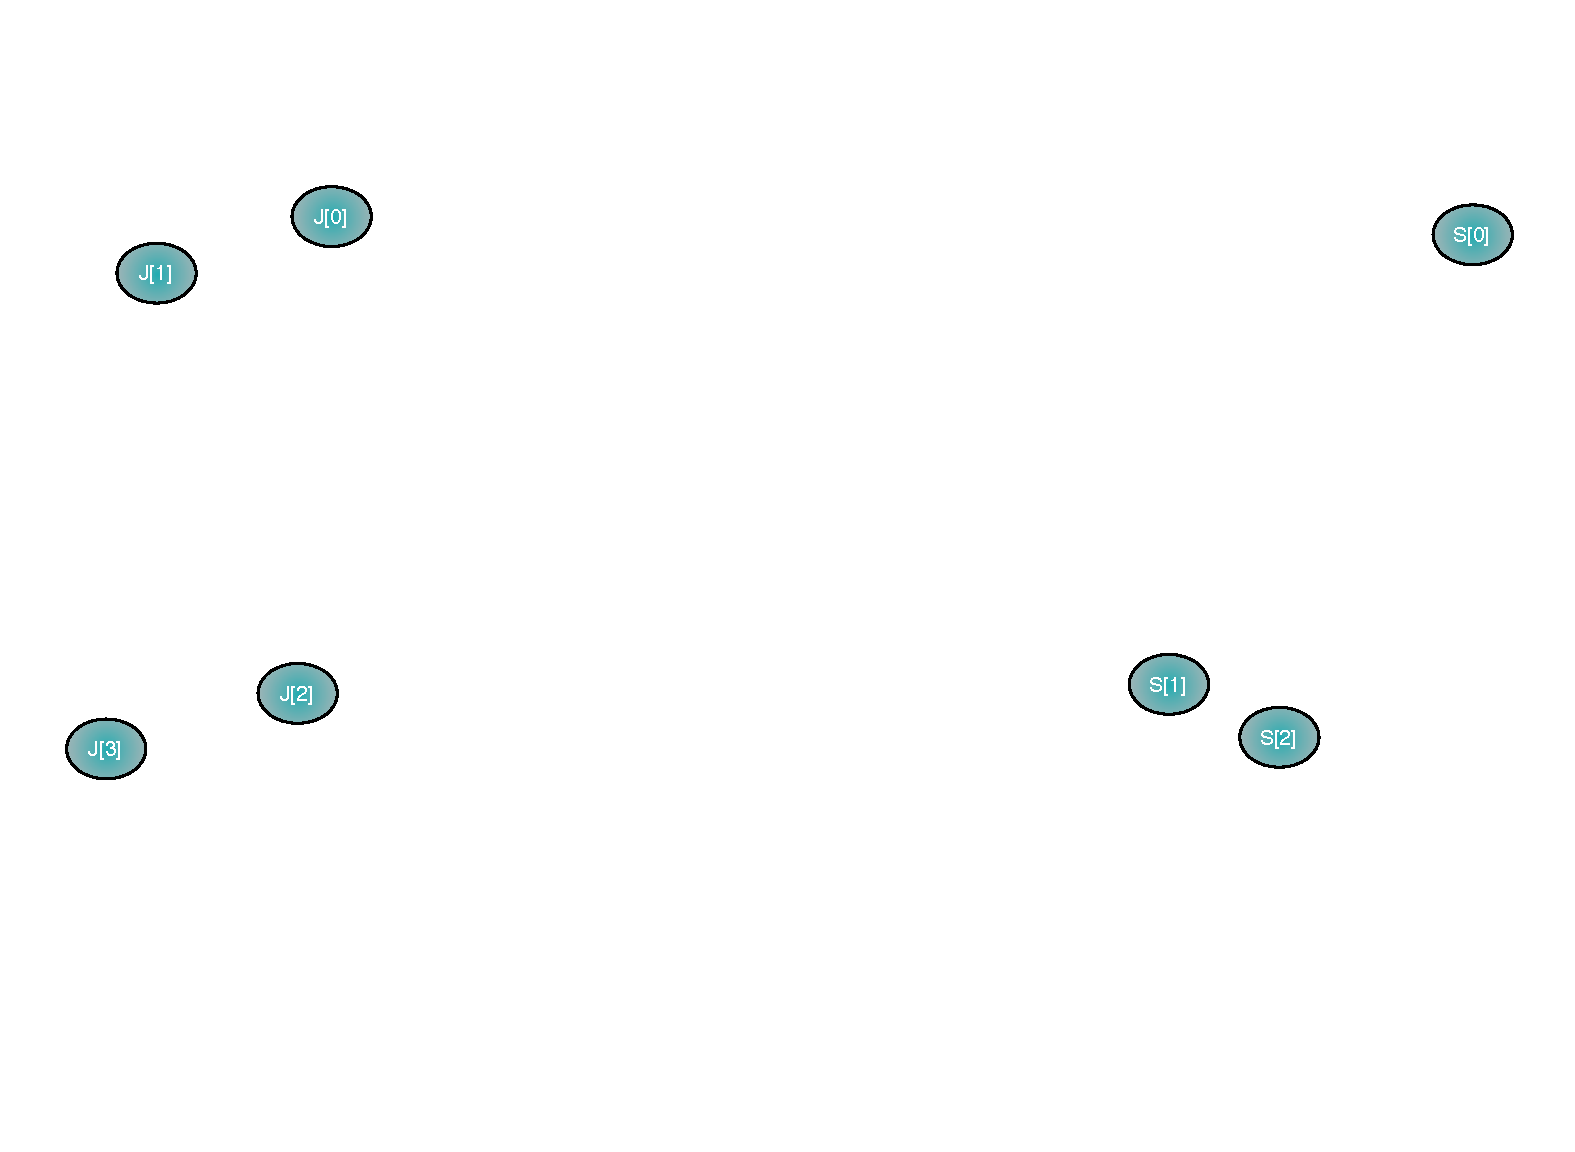
\includegraphics[width=0.9\textwidth]{../figures/progmodel/03-many-data-parallel-arrays.pdf}\end{figure}
\end{frame}


\begin{frame}
  \frametitle{Functional parallelism: via multiple classes}
  \begin{figure}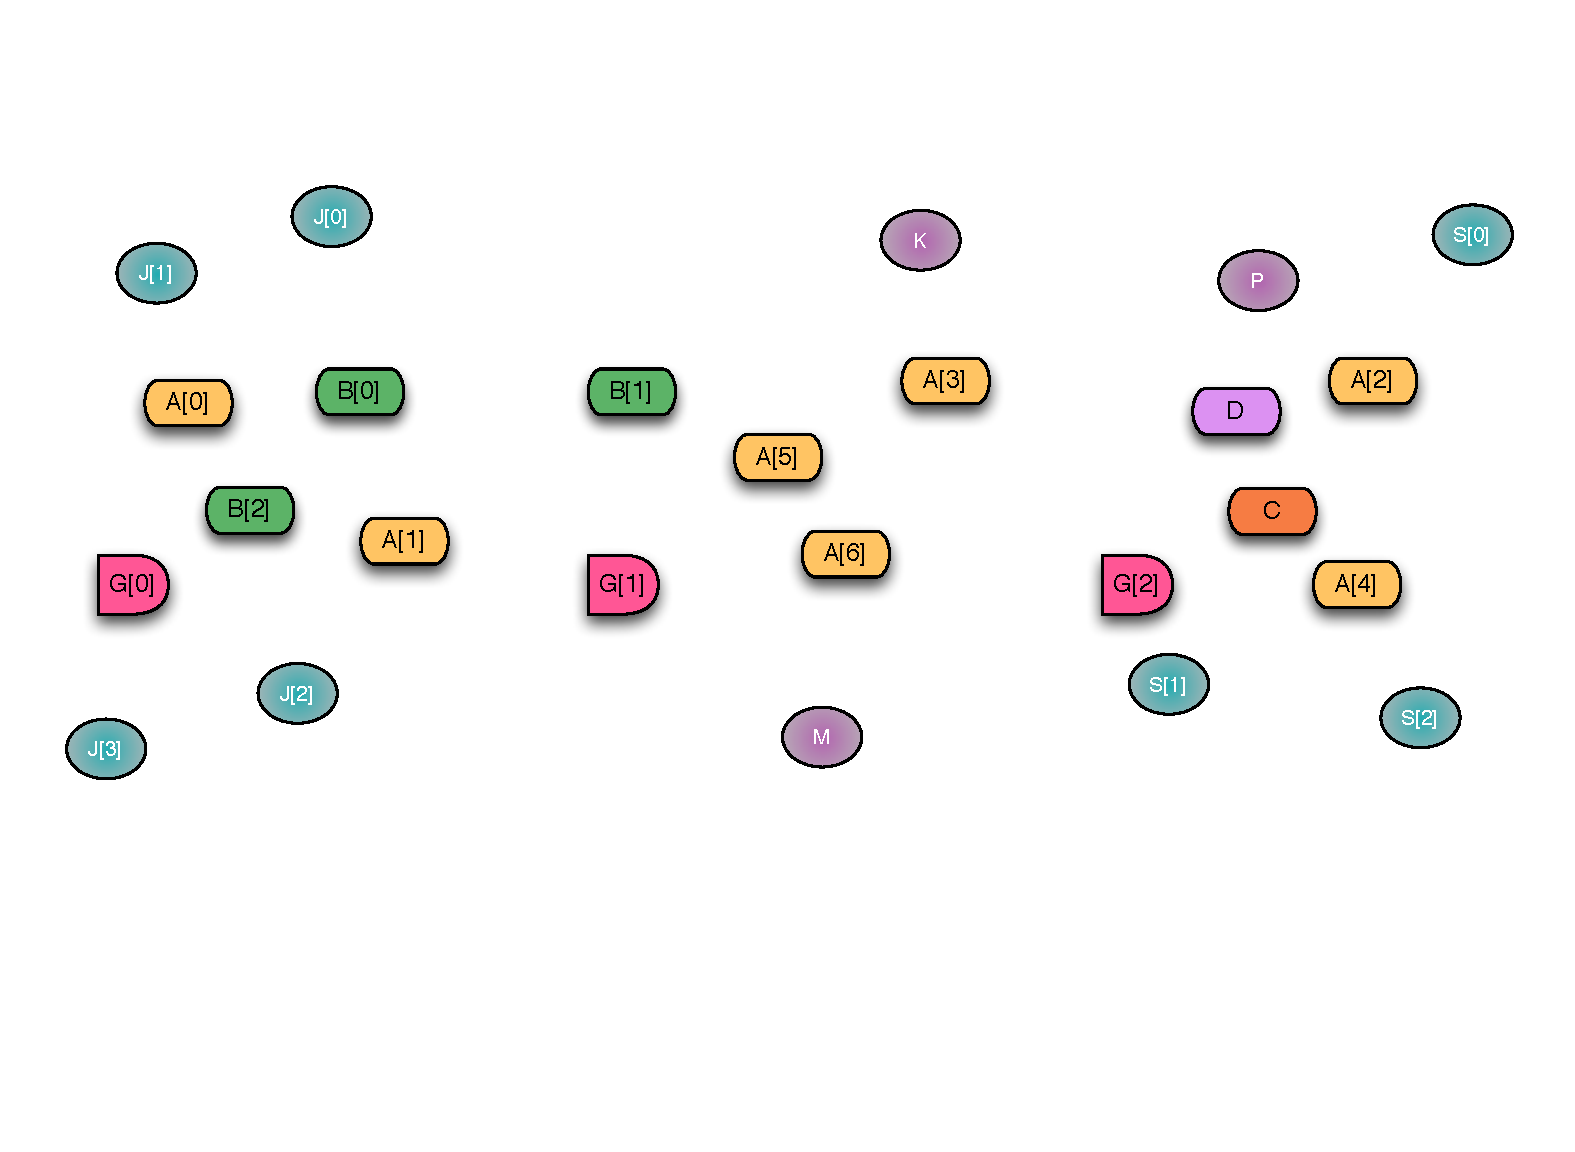
\includegraphics[width=0.9\textwidth]{../figures/progmodel/04-func-decomp-via-classes.pdf}\end{figure}
\end{frame}


\begin{frame}
  \frametitle{App logic: via classes and objects collections}
  \begin{figure}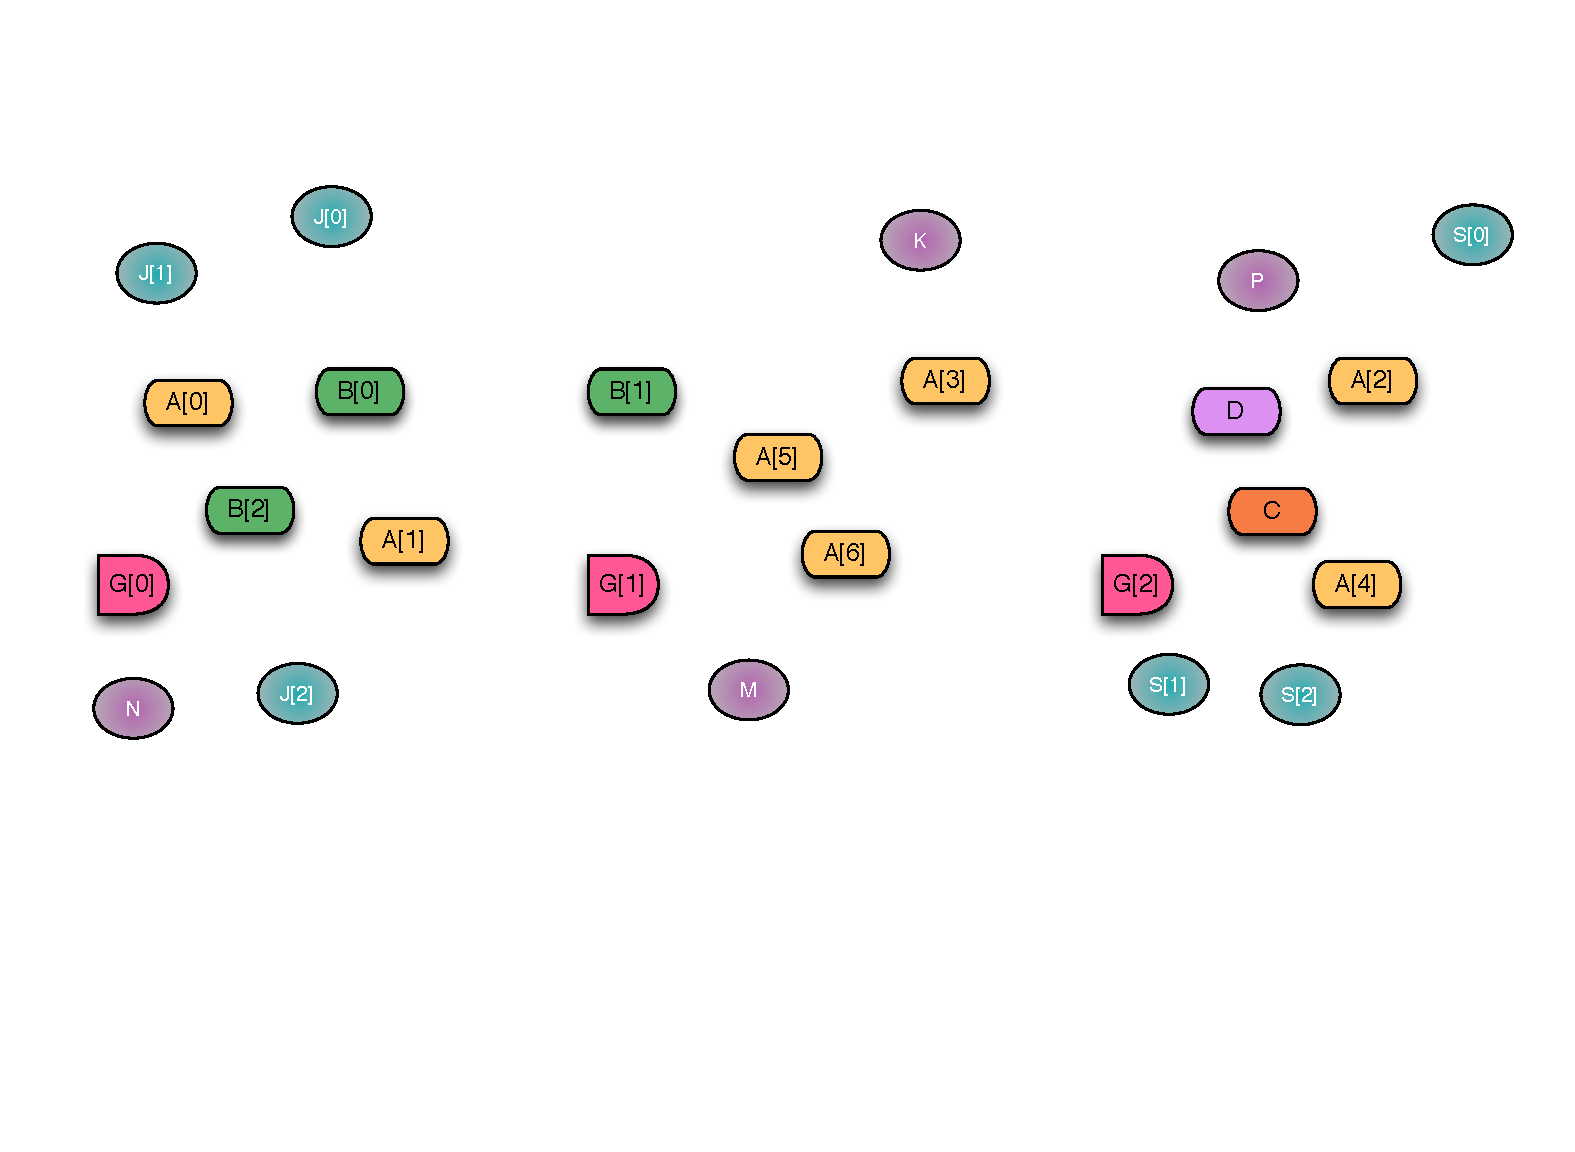
\includegraphics[width=0.9\textwidth]{../figures/progmodel/05-parallelism-via-obj-collections.pdf}\end{figure}
\end{frame}


\begin{frame}
  \frametitle{
    \only<1>{Parallelism requires distributing objects across processors}
    \only<2>{However, do not burden programmer with this view}
  }
  \begin{figure}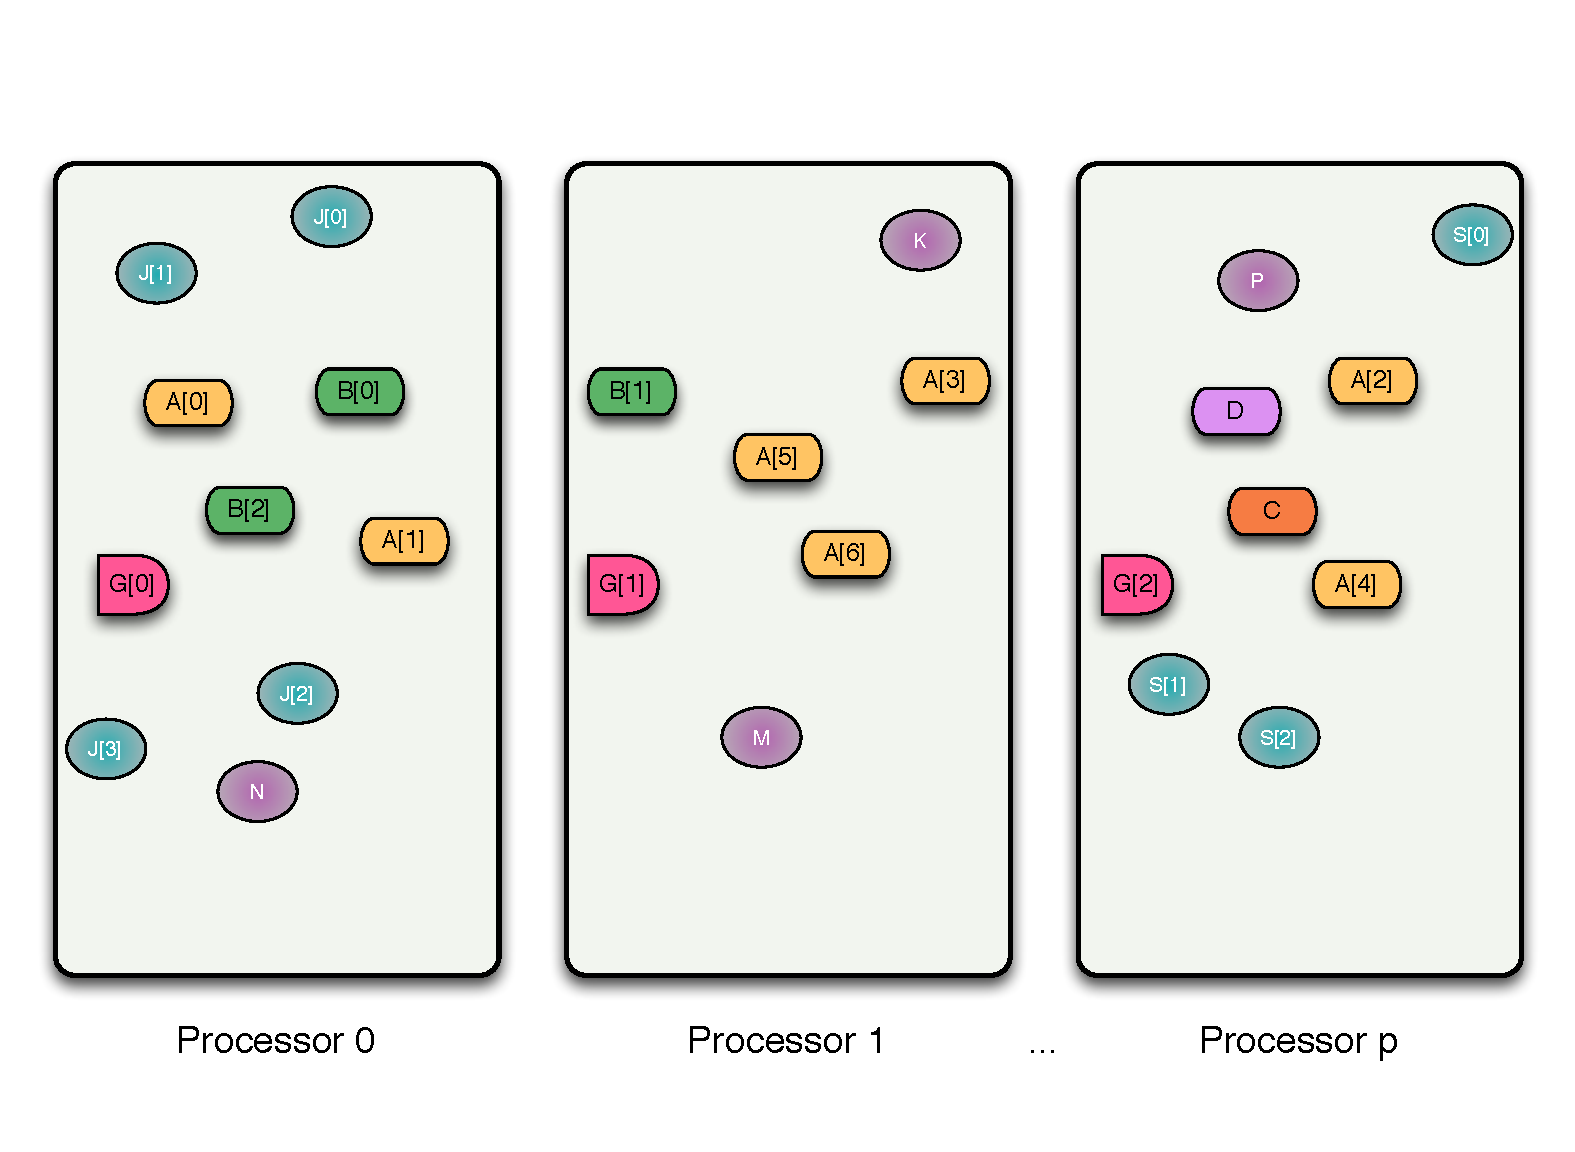
\includegraphics[width=0.9\textwidth]{../figures/progmodel/06-objects-sys-view.pdf}\end{figure}
\end{frame}


\begin{frame}
  \frametitle{
    \only<1>{Elevate some objects to global visibility}
    \only<2>{Addressing objects is independent of location}
  }
  \begin{figure}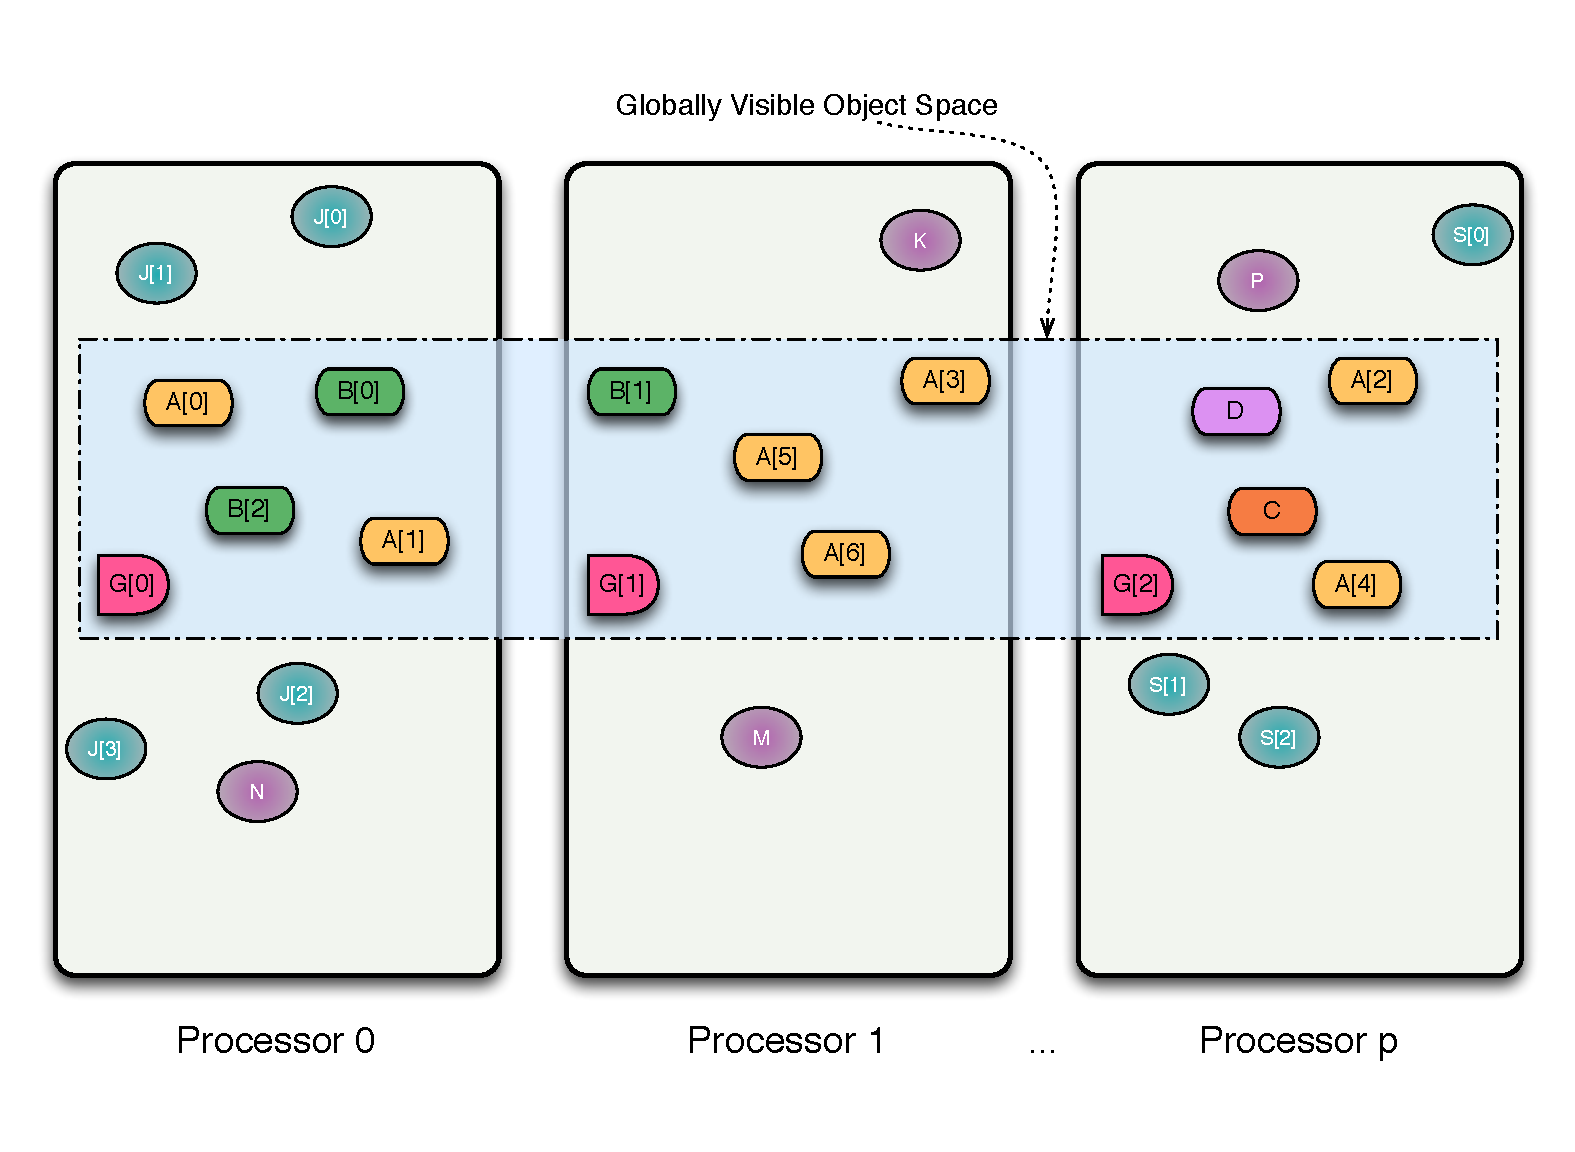
\includegraphics[width=0.9\textwidth]{../figures/progmodel/07-obj-programmer-view.pdf}\end{figure}
\end{frame}


\begin{frame}
\frametitle{Quantum Chemistry: OpenAtom}
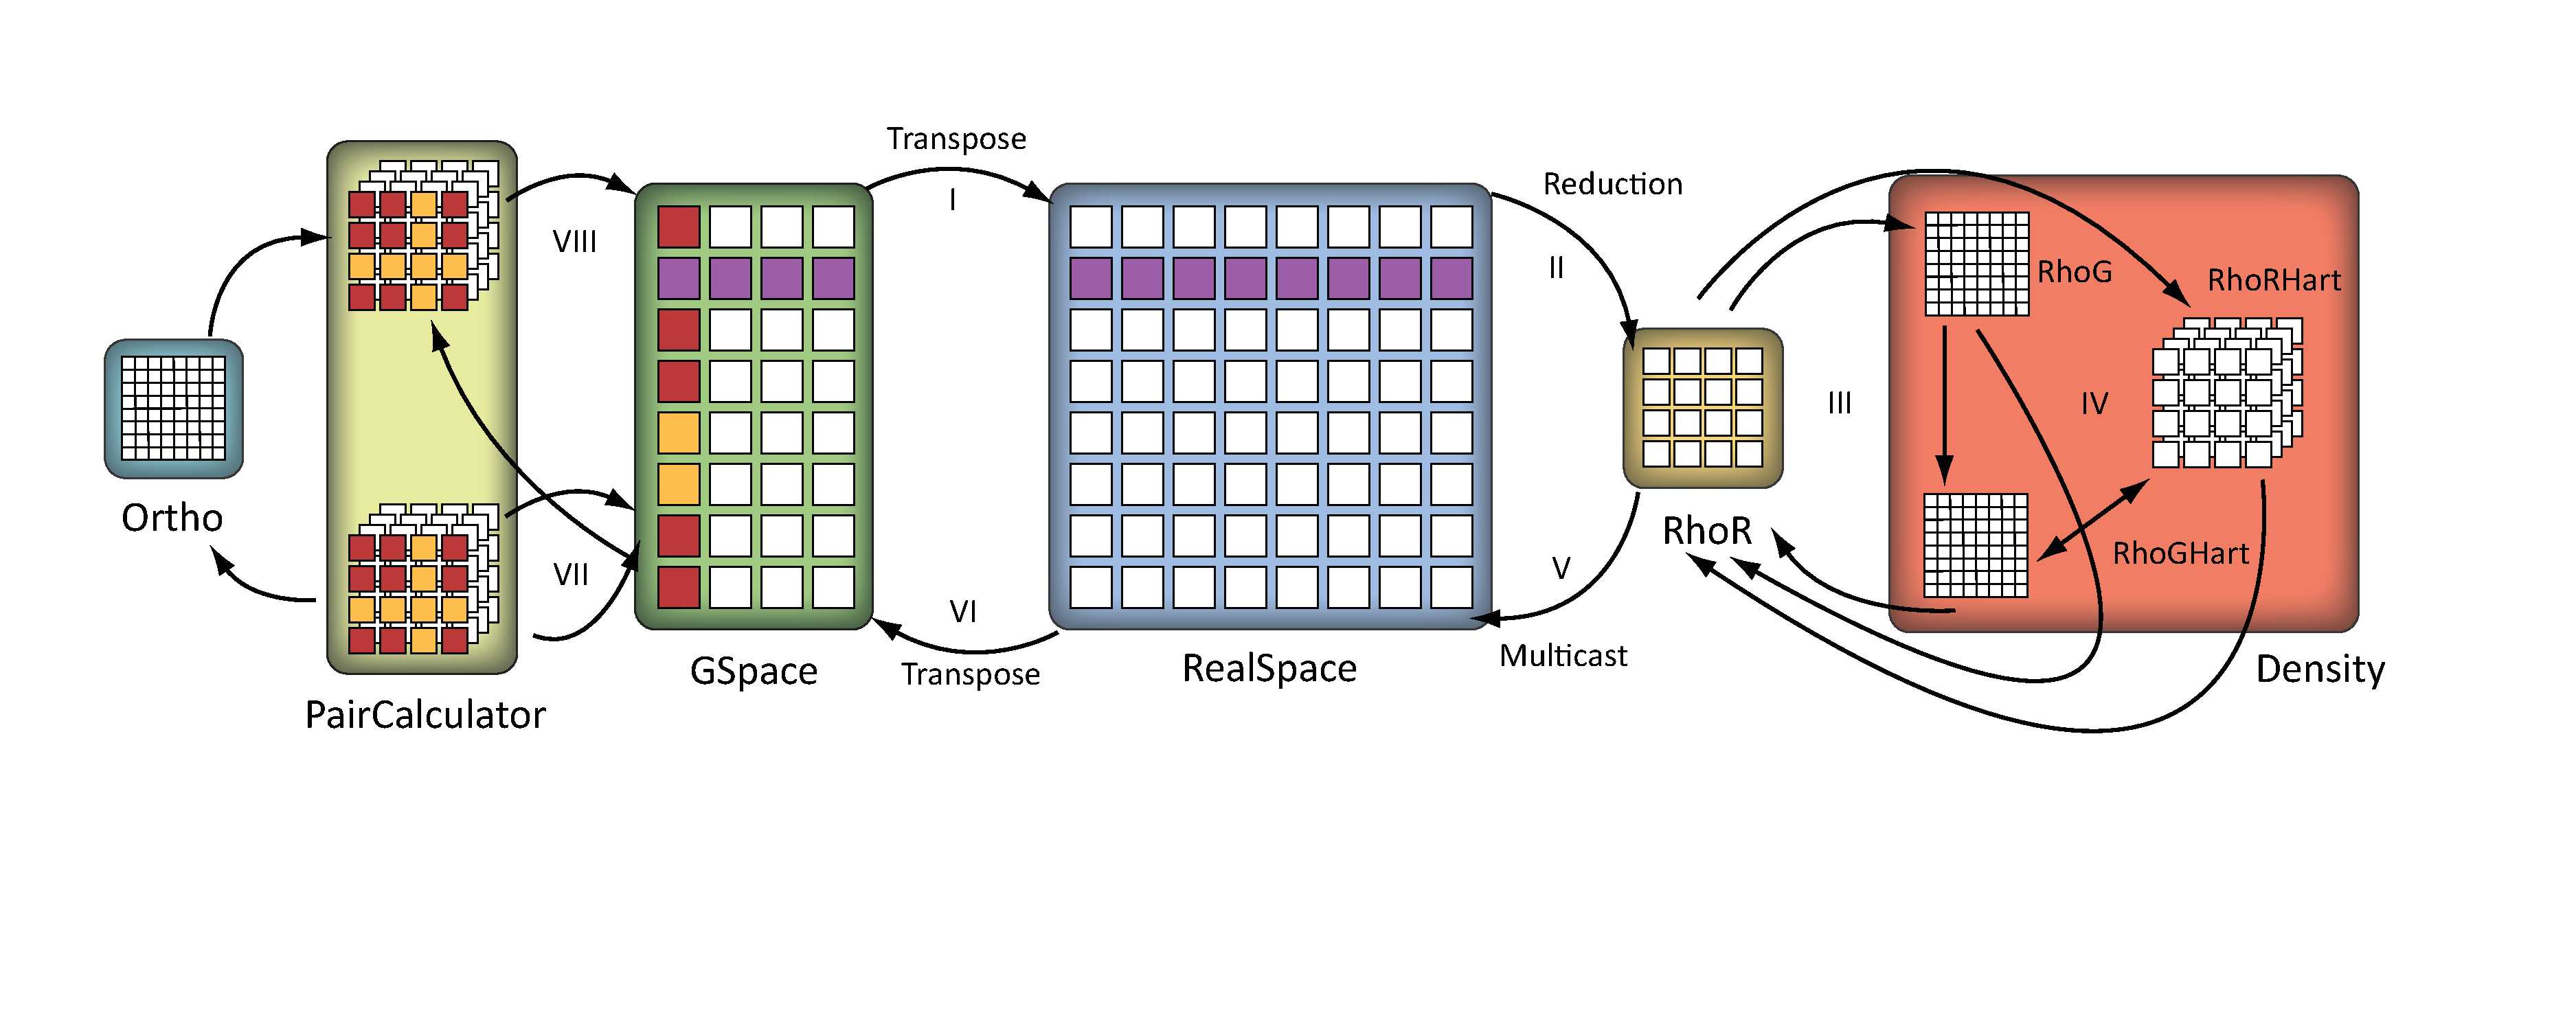
\includegraphics[width=\textwidth]{../figures/openatom/control-flow.pdf}
\end{frame}


\begin{frame}
\frametitle{Quantum Chemistry: OpenAtom}
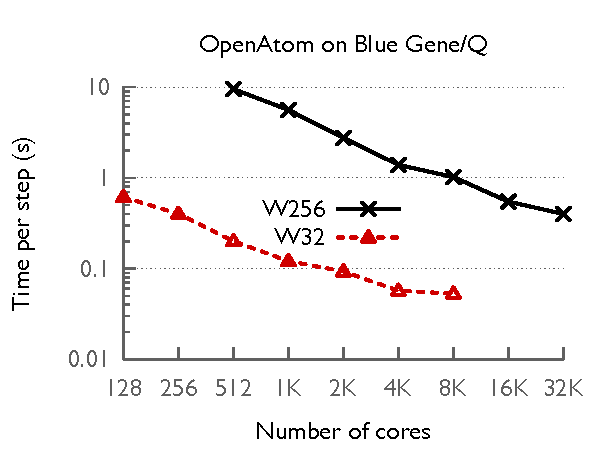
\includegraphics[width=\textwidth]{../figures/openatom/bgq.pdf}
\end{frame}


\begin{frame}
  \frametitle{}
  \begin{figure}
	\includegraphics<1>[width=0.9\textwidth]{../figures/progmodel/07-obj-programmer-view.pdf}
	\includegraphics<2>[width=0.9\textwidth]{../figures/progmodel/05-parallelism-via-obj-collections.pdf}
	\includegraphics<3>[width=0.9\textwidth]{../figures/progmodel/08-seq-obj-methods.pdf}
	\includegraphics<4>[width=0.9\textwidth]{../figures/progmodel/09-rmi-synchronous.pdf}
  \end{figure}
so far we only spoke abt units of state in the app
and expressing the app in terms of units natural to the domain
so we've done that.
we have this impressive decomposition of data and functionality across collections of objects
there's one key ingredient that i've avoided mentioning up to this point
and those are interactions.
how do you stitch all these objects into a cohesive fabric that makes the app do what its supposed
to do
these obj have to interact with each other
% 
in a sequential environment, which all of us are familiar with
app state is in objects, and app logic is via interactions. ie method invocations
%
charm retains this same modality
we enable method invocations across process or addr space boundaries
%
however with minor modifications from the sequential semantic
\end{frame}


\begin{frame}
\frametitle{1. Not every object is remotely invocable}
(1) we do NOT encourage a notion of a global address space, where it magically appears that
all app entities are in the same address space, and any object can call / interact with anyone else
instead, we strive to keep the locality information visible to the app
the first step to that is to permit RMI only on globally visible objects
  \begin{figure}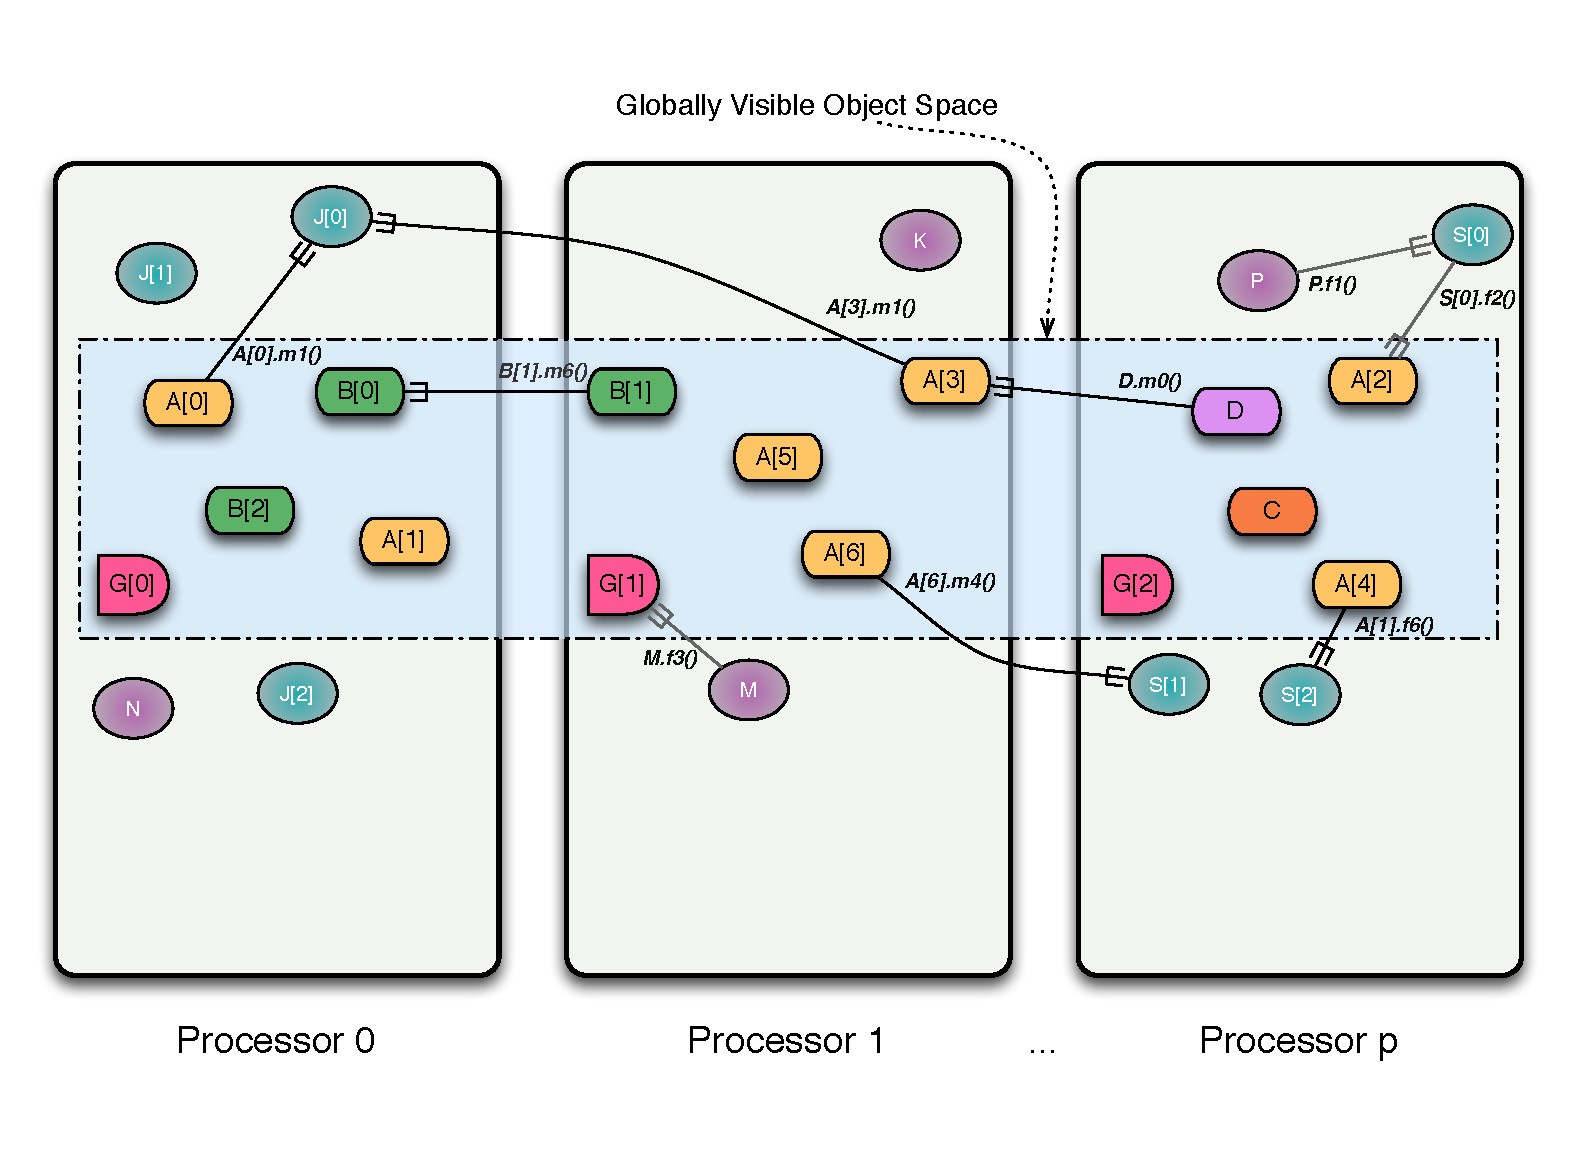
\includegraphics[width=0.9\textwidth]{../figures/progmodel/10-rmi-notgas.pdf}\end{figure}
\end{frame}


\begin{frame}
\frametitle{2. Not every method is remotely invocable}
only subset of methods elevated into global namespace
programmer annotates which methods are globally visible
only globally visible methods can be invoked across proc boundaries
intro term entry methods. will explain why later.
  \begin{figure}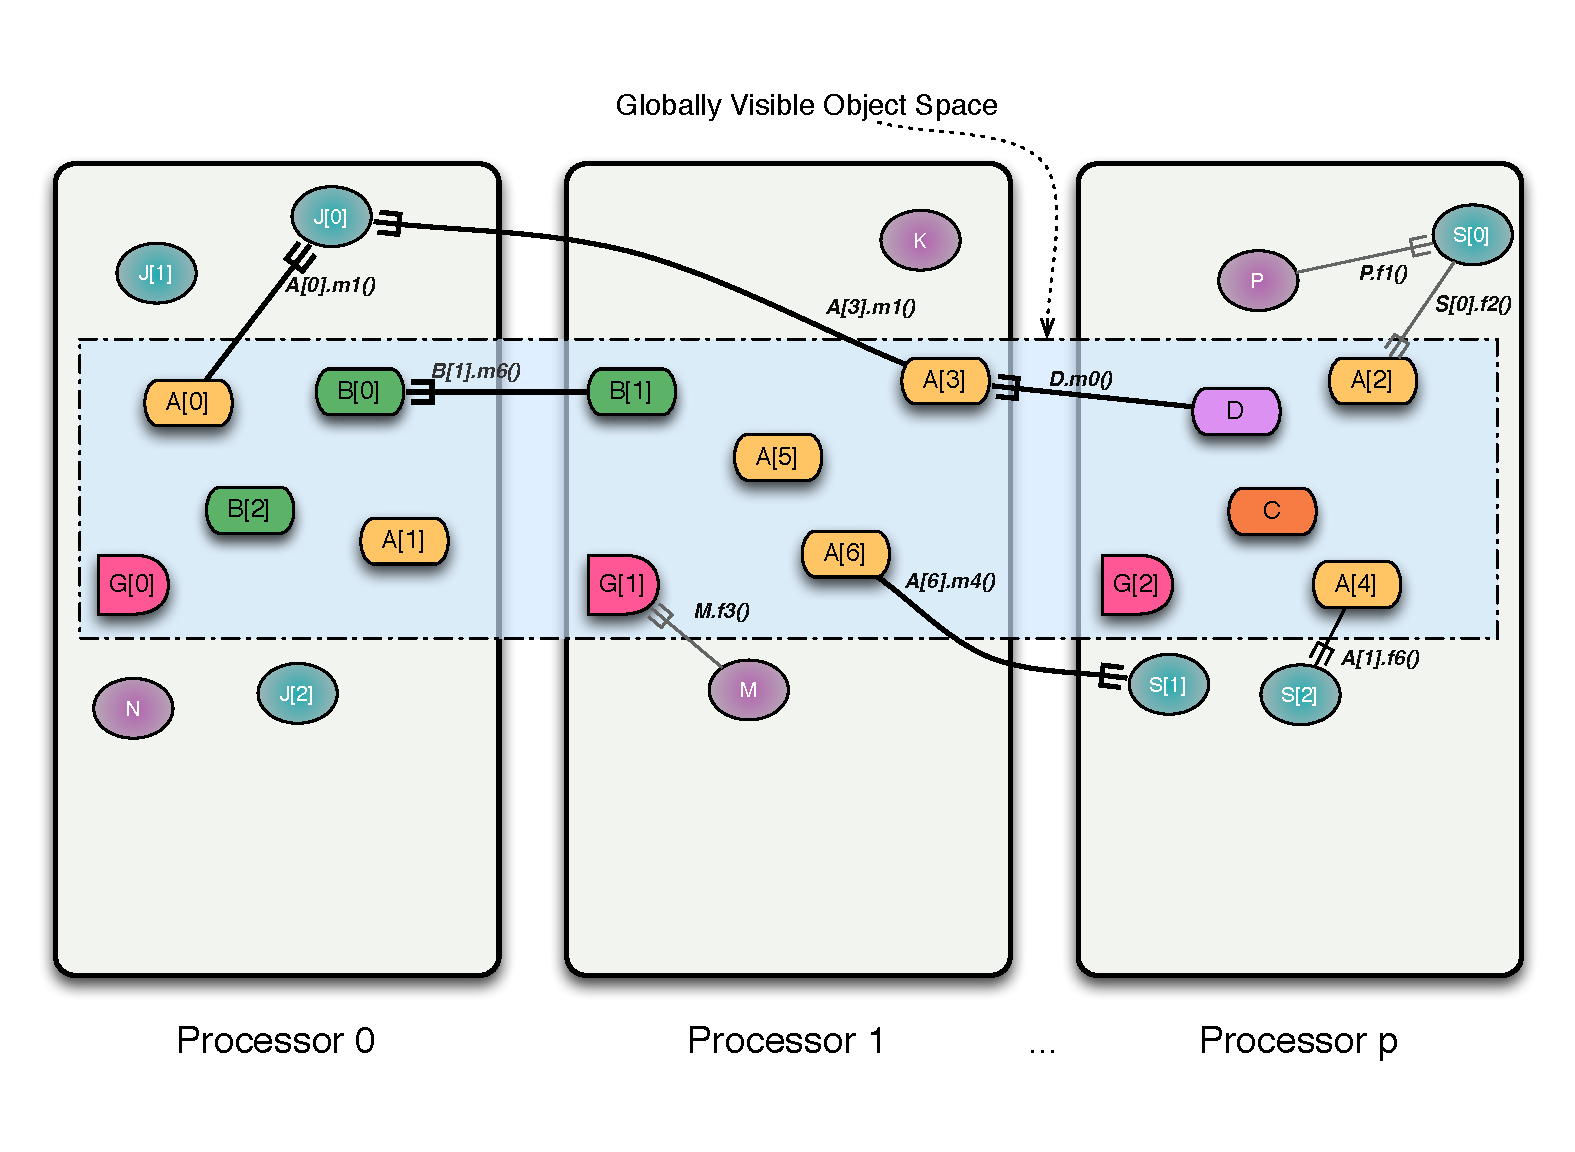
\includegraphics[width=0.9\textwidth]{../figures/progmodel/11-global-methods.pdf}\end{figure}
\end{frame}


\begin{frame}
\frametitle{3. Remote methods are of void return type}
  What happens if an object waits for a return value from a method invocation?
  \pause
  \begin{center}
    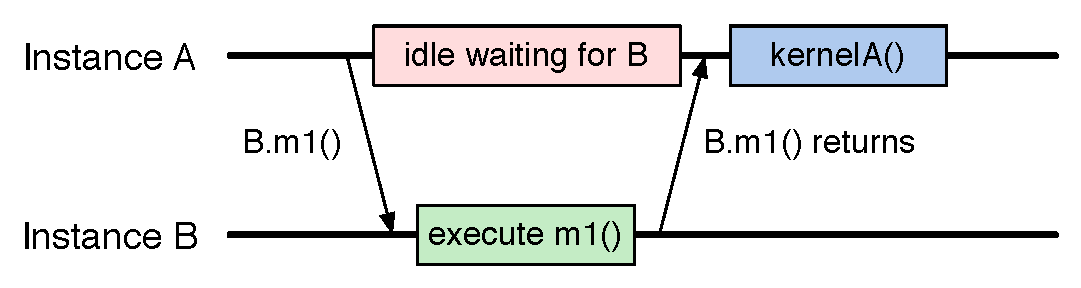
\includegraphics[width=\textwidth]{../figures/objectSequence.pdf}
  \end{center}
  \pause
  \begin{itemize}
    \item Performance
    \item Latency
    \item Reasoning about correctness
  \end{itemize}
\end{frame}


\begin{frame}
\frametitle{3. Remote methods are of void return type}
  \begin{center}
    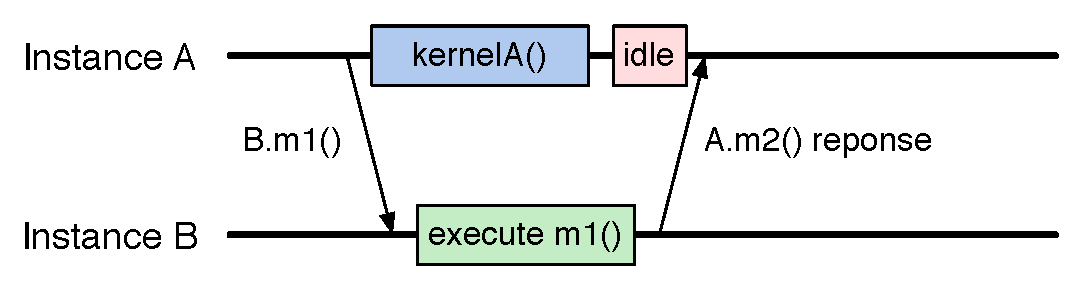
\includegraphics[width=\textwidth]{../figures/objectSequenceAsync.pdf}
  \end{center}
  \begin{itemize}
  \item Hence, method invocations should be asynchronous
    \begin{itemize}
    \item No return values
    \end{itemize}
  \item Computations are driven by the incoming data
    \begin{itemize}
    \item Initiated by the sender or method caller
    \end{itemize}
  \end{itemize}
\end{frame}



\begin{frame}
recap
    class / object - fundamental unit of state natural to parallel algo\\
    method - fundamental unit of execution in parallel algo\\
    express parallel algo interactions via methods or function calls
\end{frame}


\begin{frame}
  \frametitle{Objects interact via methods}
  \begin{figure}
    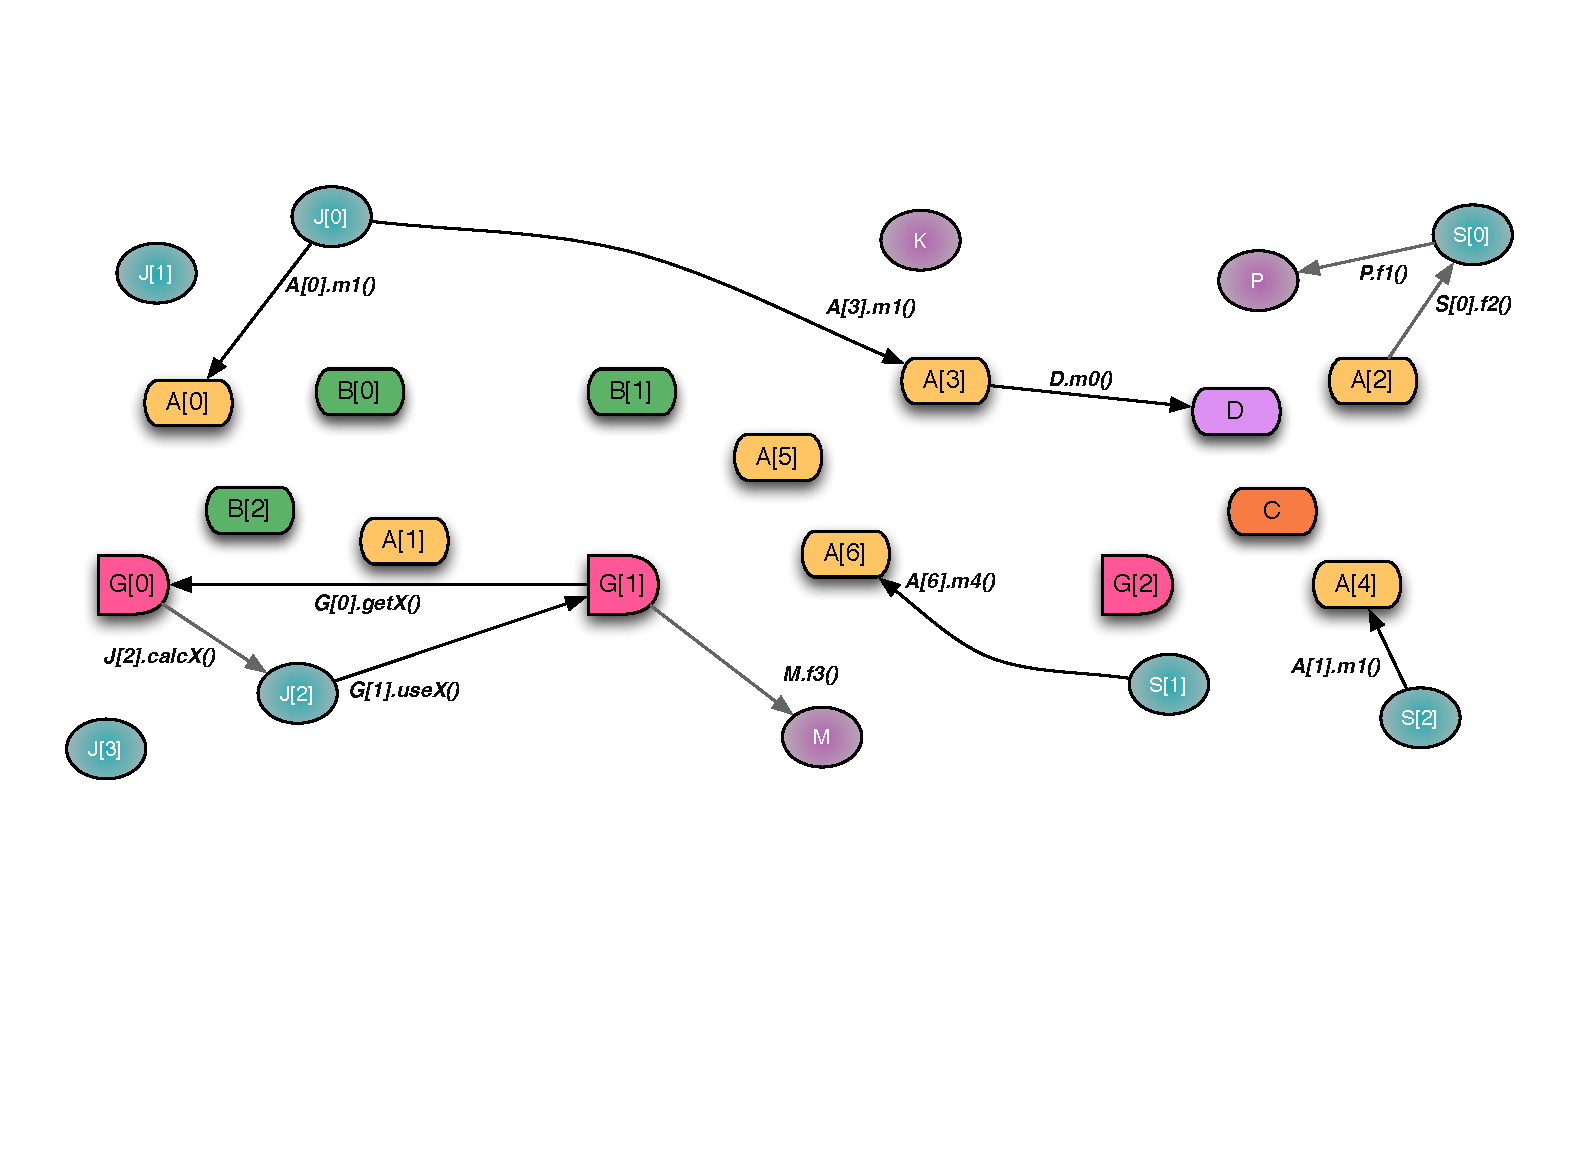
\includegraphics[width=0.9\textwidth]{../figures/progmodel/07-algo-via-objects-methods.pdf}
  \end{figure}
\end{frame}


